\documentclass{standalone}
\usepackage{tikz}
\usetikzlibrary{patterns, positioning}


\begin{document}
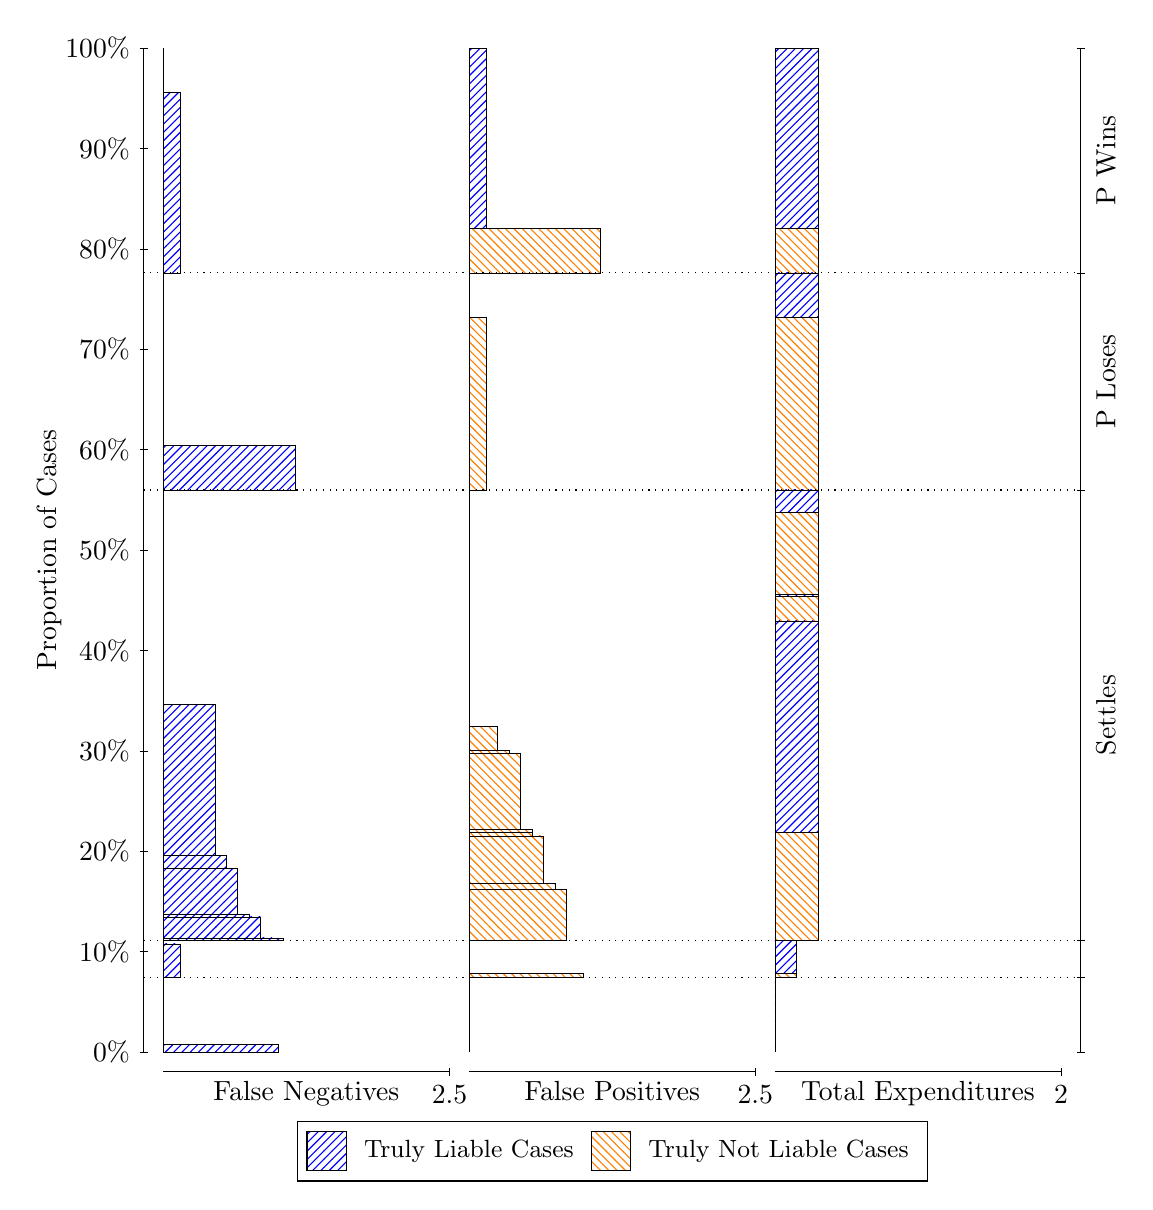
\begin{tikzpicture}
\draw[black, very thin] (1.5,1.75) -- (1.5,14.5);
\node[rotate=90, text=black, anchor=center] at (0.3, 8.125) {Proportion of Cases};
\draw[black, very thin] (1.45,1.75) -- (1.55,1.75);
\node[text=black, anchor=east] at (1.45, 1.75) {0\%};
\draw[black, very thin] (1.45,3.025) -- (1.55,3.025);
\node[text=black, anchor=east] at (1.45, 3.025) {10\%};
\draw[black, very thin] (1.45,4.3) -- (1.55,4.3);
\node[text=black, anchor=east] at (1.45, 4.3) {20\%};
\draw[black, very thin] (1.45,5.575) -- (1.55,5.575);
\node[text=black, anchor=east] at (1.45, 5.575) {30\%};
\draw[black, very thin] (1.45,6.85) -- (1.55,6.85);
\node[text=black, anchor=east] at (1.45, 6.85) {40\%};
\draw[black, very thin] (1.45,8.125) -- (1.55,8.125);
\node[text=black, anchor=east] at (1.45, 8.125) {50\%};
\draw[black, very thin] (1.45,9.4) -- (1.55,9.4);
\node[text=black, anchor=east] at (1.45, 9.4) {60\%};
\draw[black, very thin] (1.45,10.675) -- (1.55,10.675);
\node[text=black, anchor=east] at (1.45, 10.675) {70\%};
\draw[black, very thin] (1.45,11.95) -- (1.55,11.95);
\node[text=black, anchor=east] at (1.45, 11.95) {80\%};
\draw[black, very thin] (1.45,13.225) -- (1.55,13.225);
\node[text=black, anchor=east] at (1.45, 13.225) {90\%};
\draw[black, very thin] (1.45,14.5) -- (1.55,14.5);
\node[text=black, anchor=east] at (1.45, 14.5) {100\%};

\draw[black, very thin] (13.4,1.75) -- (13.4,14.5);
\draw[black, very thin] (13.35,1.75) -- (13.45,1.75);
\node[anchor=west] at (13.35, 1.75) {};
\draw[black, very thin] (13.35,2.699) -- (13.45,2.699);
\node[anchor=west] at (13.35, 2.699) {};
\draw[black, very thin] (13.35,3.17) -- (13.45,3.17);
\node[anchor=west] at (13.35, 3.17) {};
\draw[black, very thin] (13.35,8.8872) -- (13.45,8.8872);
\node[anchor=west] at (13.35, 8.8872) {};
\draw[black, very thin] (13.35,11.645) -- (13.45,11.645);
\node[anchor=west] at (13.35, 11.645) {};
\draw[black, very thin] (13.35,14.5) -- (13.45,14.5);
\node[anchor=west] at (13.35, 14.5) {};

\draw[black, very thin, pattern color=blue, pattern=north east lines] (1.75,1.75) rectangle (3.2033,1.8498);
\draw[black, very thin, pattern color=orange, pattern=north west lines] (1.75,1.8498) rectangle (1.75,2.699);
\draw[black, very thin, pattern color=blue, pattern=north east lines] (1.75,2.699) rectangle (1.968,3.1218);
\draw[black, very thin, pattern color=orange, pattern=north west lines] (1.75,3.1218) rectangle (1.75,3.17);
\draw[black, very thin, pattern color=blue, pattern=north east lines] (1.75,3.17) rectangle (3.276,3.1958);
\draw[black, very thin, pattern color=blue, pattern=north east lines] (1.75,3.1958) rectangle (3.1307,3.2);
\draw[black, very thin, pattern color=blue, pattern=north east lines] (1.75,3.2) rectangle (2.9853,3.4645);
\draw[black, very thin, pattern color=blue, pattern=north east lines] (1.75,3.4645) rectangle (2.84,3.4959);
\draw[black, very thin, pattern color=blue, pattern=north east lines] (1.75,3.4959) rectangle (2.6947,4.084);
\draw[black, very thin, pattern color=blue, pattern=north east lines] (1.75,4.084) rectangle (2.5493,4.2419);
\draw[black, very thin, pattern color=blue, pattern=north east lines] (1.75,4.2419) rectangle (2.404,6.1683);
\draw[black, very thin, pattern color=orange, pattern=north west lines] (1.75,6.1683) rectangle (1.75,8.8872);
\draw[black, very thin, pattern color=blue, pattern=north east lines] (1.75,8.8872) rectangle (3.4213,9.4523);
\draw[black, very thin, pattern color=orange, pattern=north west lines] (1.75,9.4523) rectangle (1.75,11.645);
\draw[black, very thin, pattern color=blue, pattern=north east lines] (1.75,11.645) rectangle (1.968,13.933);
\draw[black, very thin, pattern color=orange, pattern=north west lines] (1.75,13.933) rectangle (1.75,14.5);
\draw[black, very thin, pattern color=orange, pattern=north west lines] (5.6333,1.75) rectangle (5.6333,2.5991);
\draw[black, very thin, pattern color=blue, pattern=north east lines] (5.6333,2.5991) rectangle (5.6333,2.699);
\draw[black, very thin, pattern color=orange, pattern=north west lines] (5.6333,2.699) rectangle (7.0867,2.7472);
\draw[black, very thin, pattern color=blue, pattern=north east lines] (5.6333,2.7472) rectangle (5.6333,3.17);
\draw[black, very thin, pattern color=orange, pattern=north west lines] (5.6333,3.17) rectangle (6.8687,3.8137);
\draw[black, very thin, pattern color=orange, pattern=north west lines] (5.6333,3.8137) rectangle (6.7233,3.8913);
\draw[black, very thin, pattern color=orange, pattern=north west lines] (5.6333,3.8913) rectangle (6.578,4.4946);
\draw[black, very thin, pattern color=orange, pattern=north west lines] (5.6333,4.4946) rectangle (6.4327,4.534);
\draw[black, very thin, pattern color=orange, pattern=north west lines] (5.6333,4.534) rectangle (6.4327,4.5775);
\draw[black, very thin, pattern color=orange, pattern=north west lines] (5.6333,4.5775) rectangle (6.2873,5.5379);
\draw[black, very thin, pattern color=orange, pattern=north west lines] (5.6333,5.5379) rectangle (6.142,5.5764);
\draw[black, very thin, pattern color=orange, pattern=north west lines] (5.6333,5.5764) rectangle (5.9967,5.8888);
\draw[black, very thin, pattern color=blue, pattern=north east lines] (5.6333,5.8888) rectangle (5.6333,8.8872);
\draw[black, very thin, pattern color=orange, pattern=north west lines] (5.6333,8.8872) rectangle (5.8513,11.079);
\draw[black, very thin, pattern color=blue, pattern=north east lines] (5.6333,11.079) rectangle (5.6333,11.645);
\draw[black, very thin, pattern color=orange, pattern=north west lines] (5.6333,11.645) rectangle (7.3047,12.211);
\draw[black, very thin, pattern color=blue, pattern=north east lines] (5.6333,12.211) rectangle (5.8513,14.5);
\draw[black, very thin, pattern color=orange, pattern=north west lines] (9.5167,1.75) rectangle (9.5167,2.5991);
\draw[black, very thin, pattern color=blue, pattern=north east lines] (9.5167,2.5991) rectangle (9.5167,2.699);
\draw[black, very thin, pattern color=orange, pattern=north west lines] (9.5167,2.699) rectangle (9.7892,2.7472);
\draw[black, very thin, pattern color=blue, pattern=north east lines] (9.5167,2.7472) rectangle (9.7892,3.17);
\draw[black, very thin, pattern color=orange, pattern=north west lines] (9.5167,3.17) rectangle (10.062,4.534);
\draw[black, very thin, pattern color=blue, pattern=north east lines] (9.5167,4.534) rectangle (10.062,7.2242);
\draw[black, very thin, pattern color=orange, pattern=north west lines] (9.5167,7.2242) rectangle (10.062,7.5366);
\draw[black, very thin, pattern color=blue, pattern=north east lines] (9.5167,7.5366) rectangle (10.062,7.5625);
\draw[black, very thin, pattern color=orange, pattern=north west lines] (9.5167,7.5625) rectangle (10.062,8.6049);
\draw[black, very thin, pattern color=blue, pattern=north east lines] (9.5167,8.6049) rectangle (10.062,8.8872);
\draw[black, very thin, pattern color=orange, pattern=north west lines] (9.5167,8.8872) rectangle (10.062,11.079);
\draw[black, very thin, pattern color=blue, pattern=north east lines] (9.5167,11.079) rectangle (10.062,11.645);
\draw[black, very thin, pattern color=orange, pattern=north west lines] (9.5167,11.645) rectangle (10.062,12.211);
\draw[black, very thin, pattern color=blue, pattern=north east lines] (9.5167,12.211) rectangle (10.062,14.5);
\draw[black, dotted] (1.5,2.699) -- (13.4,2.699);
\draw[black, dotted] (1.5,3.17) -- (13.4,3.17);
\draw[black, dotted] (1.5,8.8872) -- (13.4,8.8872);
\draw[black, dotted] (1.5,11.645) -- (13.4,11.645);
\draw[black, very thin] (1.75,1.5) -- (5.3833,1.5);
\node[text=black, anchor=north] at (3.5667, 1.5) {False Negatives};
\draw[black, very thin] (5.3833,1.45) -- (5.3833,1.55);
\node[text=black, anchor=north] at (5.3833, 1.45) {2.5};

\draw[black, very thin] (5.6333,1.5) -- (9.2667,1.5);
\node[text=black, anchor=north] at (7.45, 1.5) {False Positives};
\draw[black, very thin] (9.2667,1.45) -- (9.2667,1.55);
\node[text=black, anchor=north] at (9.2667, 1.45) {2.5};

\draw[black, very thin] (9.5167,1.5) -- (13.15,1.5);
\node[text=black, anchor=north] at (11.333, 1.5) {Total Expenditures};
\draw[black, very thin] (13.15,1.45) -- (13.15,1.55);
\node[text=black, anchor=north] at (13.15, 1.45) {2};



\node[text=black, centered, rotate=90] at (13.72, 6.0286) {Settles};
\node[text=black, centered, rotate=90] at (13.72, 10.266) {P Loses};
\node[text=black, centered, rotate=90] at (13.72, 13.072) {P Wins};

\draw (7.449999999999999,1.5) node[draw=none] (baseCoordinate) {};
\begin{scope}[align=center]
        \matrix[scale=0.5, draw=black, below=0.5cm of baseCoordinate, nodes={draw}, column sep=0.1cm]{
            \node[rectangle, draw, minimum width=0.5cm, minimum height=0.5cm, pattern color=blue, pattern=north east lines] {}; &
            \node[draw=none, font=\small, text=black] (B) {Truly Liable Cases}; &
            \node[rectangle, draw, minimum width=0.5cm, minimum height=0.5cm, pattern color=orange, pattern=north west lines] {}; &
            \node[draw=none, font=\small, text=black] (B) {Truly Not Liable Cases}; \\
            };
\end{scope}

\end{tikzpicture}
\end{document}